\documentclass[aspectratio=169,10pt]{beamer}

\usepackage[utf8]{inputenc}
\usepackage[T1]{fontenc}
\usepackage[spanish,es-nodecimaldot]{babel}
\usepackage{lmodern}
\usepackage{microtype}
\usepackage{graphicx}
\usepackage{booktabs}
\usepackage{tabularx}
\usepackage{array}
\usepackage{tikz}
\usetikzlibrary{arrows.meta,positioning,calc,shapes.geometric}
\usepackage{ragged2e}

\graphicspath{{assets/}}

% --- Paleta ---
\definecolor{Ink}{HTML}{16213E}
\definecolor{Muted}{HTML}{64748B}
\definecolor{Paper}{HTML}{FAF7F0}
\definecolor{Blue}{HTML}{2F6690}
\definecolor{Orange}{HTML}{D97706}
\definecolor{Green}{HTML}{2F7D6D}
\definecolor{LightBlue}{HTML}{DDEAF6}
\definecolor{LightOrange}{HTML}{FDEBD3}
\definecolor{LightGreen}{HTML}{E0F1EC}
\definecolor{Line}{HTML}{D6DEE8}
\definecolor{White}{HTML}{FFFFFF}

\setbeamercolor{background canvas}{bg=Paper}
\setbeamercolor{normal text}{fg=Ink}
\setbeamercolor{frametitle}{fg=Ink,bg=Paper}
\setbeamercolor{footline}{fg=Muted,bg=Paper}
\setbeamerfont{frametitle}{size=\Large,series=\bfseries}
\setbeamerfont{framesubtitle}{size=\small,series=\mdseries}
\setbeamerfont{footline}{size=\scriptsize}
\setbeamertemplate{navigation symbols}{}
\setbeamertemplate{itemize item}{\color{Orange}$\blacktriangleright$}
\setbeamertemplate{itemize subitem}{\color{Blue}$\bullet$}
\setlength{\parskip}{0.25em}

\setbeamertemplate{frametitle}{%
  \vspace{0.15cm}
  \begin{beamercolorbox}[wd=\paperwidth,leftskip=0.55cm,rightskip=0.55cm,sep=0.18cm]{frametitle}
    \insertframetitle\par
    {\usebeamerfont{framesubtitle}\color{Muted}\insertframesubtitle}
  \end{beamercolorbox}
  \vspace{-0.25cm}
  \hspace{0.55cm}\color{Line}\rule{0.91\paperwidth}{0.6pt}
}

\setbeamertemplate{footline}{%
  \hbox{%
  \begin{beamercolorbox}[wd=.79\paperwidth,ht=2.2ex,dp=1.1ex,leftskip=.55cm]{footline}%
    Sueño y memoria - TP Neurociencias del Desarrollo Productivo
  \end{beamercolorbox}%
  \begin{beamercolorbox}[wd=.21\paperwidth,ht=2.2ex,dp=1.1ex,rightskip=.55cm]{footline}%
    \hfill\insertframenumber/\inserttotalframenumber
  \end{beamercolorbox}}
}

\newcommand{\source}[1]{\vfill {\tiny\color{Muted}Fuente: #1}}
\newcommand{\claim}[1]{\vspace{0.15cm}{\large\bfseries\color{Ink}#1}\par\vspace{0.25cm}}
\newcommand{\smallnote}[1]{{\scriptsize\color{Muted}#1}}
\newcommand{\metric}[3]{%
  \begin{beamercolorbox}[wd=#1,sep=0.22cm,rounded=true]{metricbox}
  {\Large\bfseries\color{#2}#3}\par
  \end{beamercolorbox}}
\setbeamercolor{metricbox}{bg=White,fg=Ink}
\setbeamercolor{bluecard}{bg=LightBlue,fg=Ink}
\setbeamercolor{orangecard}{bg=LightOrange,fg=Ink}
\setbeamercolor{greencard}{bg=LightGreen,fg=Ink}
\setbeamercolor{whitecard}{bg=White,fg=Ink}
\setbeamercolor{darkcard}{bg=Ink,fg=White}

\newenvironment{card}[2][whitecard]{%
  \begin{beamercolorbox}[wd=#2,sep=0.20cm,rounded=true]{#1}\RaggedRight
}{\end{beamercolorbox}}

\title{Sueño, memoria y señales fisiológicas}
\subtitle{¿Mejora el sueño la consolidación de la memoria declarativa?}
\author{Keoni Dubovitsky \;\textbullet\; Joaquín Pelufo \;\textbullet\; Sergio Tenoch Sil Cruz}
\date{Trabajo práctico - Neurociencias del Desarrollo Productivo - 18/6/2026}

\begin{document}

% 1
{\setbeamercolor{background canvas}{bg=Ink}
\begin{frame}[plain]
\begin{tikzpicture}[remember picture,overlay]
  \draw[Blue, line width=1.5pt, opacity=.9] ($(current page.south west)+(0.7,1.0)$) .. controls +(2.8,1.2) and +(-2.2,-1.2) .. ($(current page.south east)+(-0.7,2.2)$);
  \draw[Orange, line width=1.0pt, opacity=.9] ($(current page.south west)+(1.1,0.55)$) .. controls +(2.2,1.0) and +(-3.0,-.9) .. ($(current page.south east)+(-0.8,1.3)$);
  \fill[Blue, opacity=.13] ($(current page.north east)+(-3.5,-1.5)$) circle (2.0);
\end{tikzpicture}
\vspace{0.85cm}
{\color{White}\Huge\bfseries Sueño, memoria y señales fisiológicas}\par\vspace{0.30cm}
{\color{LightBlue}\Large ¿Mejora el sueño la consolidación de la memoria declarativa?}\par
\vspace{0.70cm}
\begin{beamercolorbox}[wd=0.75\paperwidth,sep=0.28cm,rounded=true]{darkcard}
\Large Tesis oral: evidencia compatible con la hipótesis, como apoyo descriptivo y parcial.
\end{beamercolorbox}
\vfill
{\color{White}\normalsize Keoni Dubovitsky \;\textbullet\; Joaquín Pelufo \;\textbullet\; Sergio Tenoch Sil Cruz}\par
{\color{LightBlue}\small Trabajo práctico - Neurociencias del Desarrollo Productivo - 18/6/2026}
\end{frame}
}

% 2
\begin{frame}{Respuesta en 30 segundos}{La idea principal se mantiene: sueño como posible aliado de la consolidación declarativa.}
\begin{columns}[T,totalwidth=\textwidth]
\begin{column}{0.32\textwidth}
\begin{card}[bluecard]{\linewidth}
{\bfseries Pregunta}\par
¿Dormir después de aprender asociaciones palabra-definición mejora el recuerdo posterior?
\end{card}
\end{column}
\begin{column}{0.32\textwidth}
\begin{card}[orangecard]{\linewidth}
{\bfseries Hallazgo}\par
El sujeto en condición sueño alcanzó \textbf{17/20} palabras en TS y mostró mejora \textbf{+2} desde TR.
\end{card}
\end{column}
\begin{column}{0.32\textwidth}
\begin{card}[greencard]{\linewidth}
{\bfseries Cautela}\par
El EEG con sueño es secundario; memoria y fisiología se integran teóricamente, no como correlación directa.
\end{card}
\end{column}
\end{columns}
\vspace{0.65cm}
\claim{Conclusión breve: compatible con consolidación durante el sueño; no es una demostración causal.}
\source{Consigna oficial del TP; análisis propio de planilla de memoria y dataset BrainVision secundario.}
\end{frame}

% 3
\begin{frame}{Diseño: aprender, esperar y volver a evaluar}{Dos condiciones, tres etapas y una lectura descriptiva.}
\begin{center}
\begin{tikzpicture}[node distance=1.25cm, every node/.style={font=\small}]
\node[draw=Blue, rounded corners, fill=LightBlue, minimum width=2.5cm, minimum height=1.0cm, align=center] (tr) {\textbf{TR}\ Línea de base\\20 asociaciones};
\node[draw=Orange, rounded corners, fill=LightOrange, minimum width=3.1cm, minimum height=1.0cm, align=center, right=2.1cm of tr, yshift=0.65cm] (sleep) {\textbf{Sueño}\ siesta prevista\\$\sim$90 min};
\node[draw=Muted, rounded corners, fill=White, minimum width=3.1cm, minimum height=1.0cm, align=center, right=2.1cm of tr, yshift=-0.65cm] (wake) {\textbf{Control}\ vigilia\\despiertos};
\node[draw=Green, rounded corners, fill=LightGreen, minimum width=2.7cm, minimum height=1.0cm, align=center, right=2.4cm of sleep, yshift=-0.65cm] (ts) {\textbf{TS}\ evaluación\\final};
\draw[-{Stealth[length=3mm]}, line width=1.1pt, color=Muted] (tr.east) -- (sleep.west);
\draw[-{Stealth[length=3mm]}, line width=1.1pt, color=Muted] (tr.east) -- (wake.west);
\draw[-{Stealth[length=3mm]}, line width=1.1pt, color=Muted] (sleep.east) -- (ts.west);
\draw[-{Stealth[length=3mm]}, line width=1.1pt, color=Muted] (wake.east) -- (ts.west);
\end{tikzpicture}
\end{center}
\vspace{0.25cm}
\begin{columns}[T,totalwidth=\textwidth]
\begin{column}{0.49\textwidth}
\begin{card}[whitecard]{\linewidth}
\textbf{Variable de interés}\par
Cambio TR$\rightarrow$TS y desempeño final en la tarea de memoria declarativa.
\end{card}
\end{column}
\begin{column}{0.49\textwidth}
\begin{card}[whitecard]{\linewidth}
\textbf{Alcance inferencial}\par
El grupo sueño tiene $n=1$: se reporta patrón descriptivo, no estadística fuerte.
\end{card}
\end{column}
\end{columns}
\source{Planilla de tarea de palabras; guion metodológico del práctico.}
\end{frame}

% 4
\begin{frame}{Dos fuentes de datos: una regla}{La fisiología del sueño y la memoria no se tratan como si fueran del mismo sujeto.}
\small
\begin{columns}[T,totalwidth=\textwidth]
\begin{column}{0.56\textwidth}
\begin{card}[whitecard]{\linewidth}
\begin{tabularx}{\linewidth}{>{\bfseries}lX}
\toprule
Fuente & Uso y restricción\\
\midrule
Memoria & Planilla de palabras: 4 sujetos, 3 vigilia y 1 sueño; se usa para TR/TS.\\
EEG & BrainVision secundario de una persona que sí durmió; se usa para hipnograma y bandas.\\
OpenBCI & Sujeto propio no durmió; se usa como limitación y discusión.\\
\bottomrule
\end{tabularx}
\end{card}
\vspace{0.20cm}
\begin{card}[greencard]{\linewidth}
\textbf{Regla metodológica:} no mezclar memoria y EEG como si fueran mismo sujeto o sesión.
\end{card}
\end{column}
\begin{column}{0.40\textwidth}
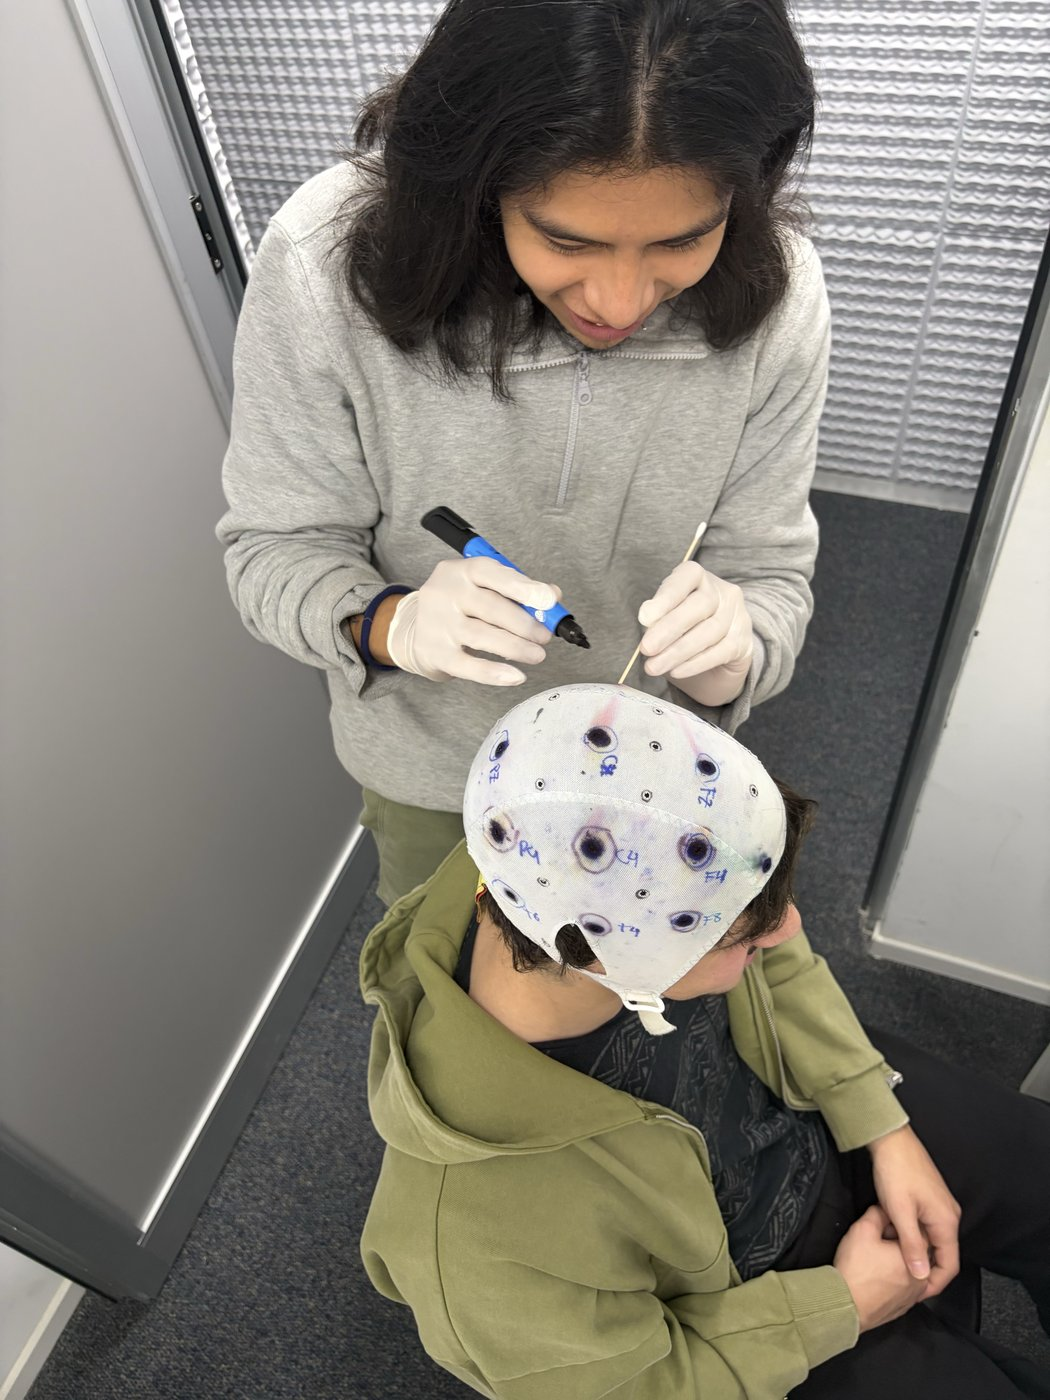
\includegraphics[height=0.52\textheight]{openbci_procedimiento.png}\par
\smallnote{Foto del procedimiento propio; no es el EEG analizado.}
\end{column}
\end{columns}
\source{README del trabajo; regla metodológica de la cátedra; foto del procedimiento propio.}
\end{frame}

% 5
\begin{frame}{Qué esperábamos encontrar}{Predicciones definidas antes de interpretar los resultados.}
\begin{columns}[T,totalwidth=\textwidth]
\begin{column}{0.31\textwidth}
\begin{card}[bluecard]{\linewidth}
{\bfseries 1. Conducta}\par
Mayor retención TR$\rightarrow$TS o mejor desempeño final tras dormir.
\end{card}
\end{column}
\begin{column}{0.31\textwidth}
\begin{card}[orangecard]{\linewidth}
{\bfseries 2. Fisiología}\par
Arquitectura NREM con sueño profundo, idealmente SWS.
\end{card}
\end{column}
\begin{column}{0.31\textwidth}
\begin{card}[greencard]{\linewidth}
{\bfseries 3. Mecanismo}\par
Delta, sigma/husos y ripples como ritmos ligados a consolidación activa.
\end{card}
\end{column}
\end{columns}
\vspace{0.7cm}
\begin{card}[whitecard]{\textwidth}
\textbf{Criterio de decisión:} la hipótesis se considera apoyada si el patrón conductual y la arquitectura fisiológica son compatibles. Se evita decir ``demostrado'' por el tamaño muestral y la separación de fuentes.
\end{card}
\source{Clase 3 - Sueño y Memoria; consigna oficial del TP.}
\end{frame}

% 6
\begin{frame}{Marco teórico aplicado}{El foco no es ``dormir descansó'', sino qué hace el NREM con las memorias.}
\small
\begin{columns}[T,totalwidth=\textwidth]
\begin{column}{0.57\textwidth}
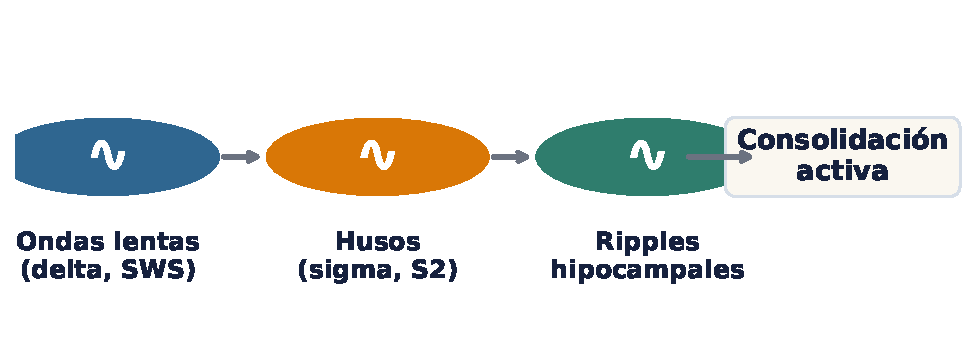
\includegraphics[width=\linewidth]{mecanismo_oscilaciones.pdf}
\vspace{0.10cm}
\begin{card}[whitecard]{\linewidth}
\textbf{Consolidación activa:} en NREM se reactivan memorias dependientes del hipocampo y se favorece su integración neocortical.
\end{card}
\end{column}
\begin{column}{0.39\textwidth}
\begin{card}[bluecard]{\linewidth}
\textbf{Ondas lentas}\par
Delta dominante en SWS; organiza ventanas de reactivación.
\end{card}
\vspace{0.18cm}
\begin{card}[orangecard]{\linewidth}
\textbf{Husos / sigma}\par
Ritmos talamocorticales en S2; aquí se usa sigma como proxy.
\end{card}
\vspace{0.18cm}
\begin{card}[greencard]{\linewidth}
\textbf{Homeostasis}\par
El sueño puede mejorar señal/ruido al reajustar pesos sinápticos.
\end{card}
\end{column}
\end{columns}
\source{Clase 3 - Sueño y Memoria; consolidación activa y homeostasis sináptica.}
\end{frame}

% 7
\begin{frame}{Métodos: dos análisis complementarios}{Conducta para memoria; EEG para fisiología del sueño.}
\begin{columns}[T,totalwidth=\textwidth]
\begin{column}{0.49\textwidth}
\begin{card}[bluecard]{\linewidth}
\textbf{Tarea de palabras}\par
\begin{itemize}
\item 20 asociaciones palabra rara-definición.
\item TR como línea de base; TS como test final.
\item Dos puntajes: palabra exacta y definición semántica.
\end{itemize}
\end{card}
\end{column}
\begin{column}{0.49\textwidth}
\begin{card}[orangecard]{\linewidth}
\textbf{EEG secundario}\par
\begin{itemize}
\item BrainVision, 10 canales, 250 Hz.
\item Filtros: notch 50 Hz + pasa banda 0.3-35 Hz.
\item Épocas de 30 s alineadas al scoring.
\end{itemize}
\end{card}
\end{column}
\end{columns}
\vspace{0.4cm}
\begin{card}[whitecard]{\textwidth}
\textbf{Decisión crítica:} C4 se descartó por artefactos; el análisis espectral se reporta sobre C3, que pasó el control de calidad.
\end{card}
\source{Planilla de memoria; Clase 9 - EEG; análisis MNE del dataset BrainVision.}
\end{frame}

% 8
\begin{frame}{Resultado conductual: memoria}{El sujeto sueño tuvo el mayor desempeño final, pero ya partía alto.}
\begin{columns}[T,totalwidth=\textwidth]
\begin{column}{0.64\textwidth}
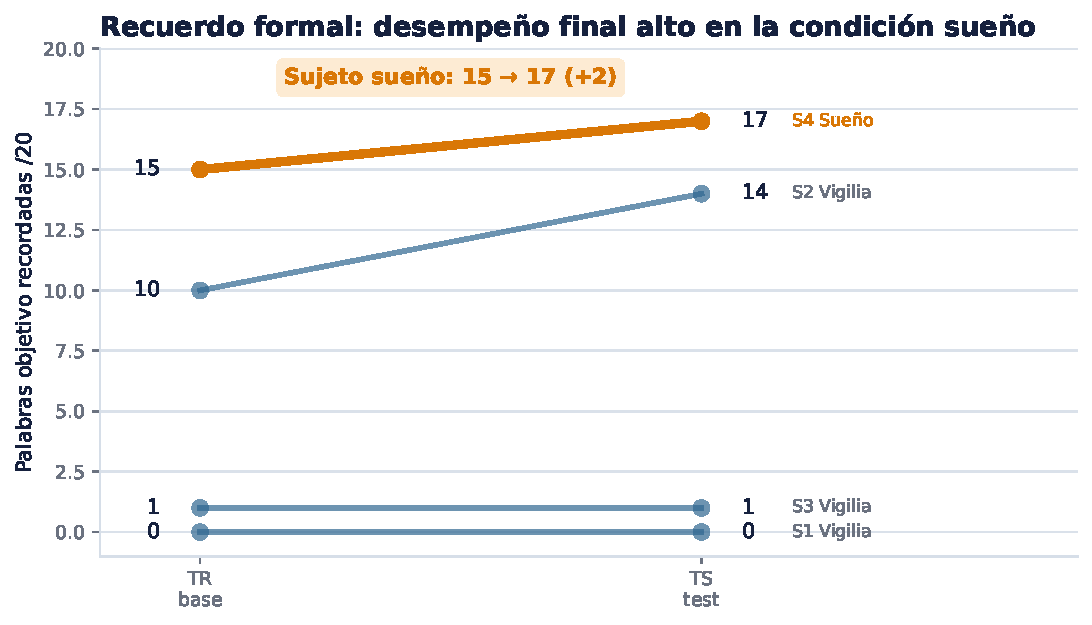
\includegraphics[width=\linewidth]{memoria_tr_ts.pdf}
\end{column}
\begin{column}{0.33\textwidth}
\begin{card}[orangecard]{\linewidth}
\textbf{Lectura principal}\par
Sujeto sueño: 15/20 en TR y 17/20 en TS.
\end{card}
\vspace{0.25cm}
\begin{card}[bluecard]{\linewidth}
\textbf{Lo descriptivo}\par
TS alto y mejora +2; compatible con la hipótesis.
\end{card}
\vspace{0.25cm}
\begin{card}[whitecard]{\linewidth}
\textbf{Lo que limita}\par
No prueba causal: $n=1$ y línea de base inicial alta.
\end{card}
\end{column}
\end{columns}
\source{Planilla PRACTICO LABORATORIO EQUIPO 1.xlsx; scoring reproducible de memoria.}
\end{frame}

% 9
\begin{frame}{EEG: limpieza antes de interpretación}{El procesamiento evita confundir ruido con fisiología.}
\begin{columns}[T,totalwidth=\textwidth]
\begin{column}{0.55\textwidth}
\begin{tikzpicture}[node distance=0.55cm, every node/.style={font=\small}]
\node[draw=Blue, rounded corners, fill=LightBlue, minimum width=5.7cm, minimum height=.65cm, align=center] (a) {Lectura BrainVision con MNE};
\node[draw=Blue, rounded corners, fill=LightBlue, minimum width=5.7cm, minimum height=.65cm, align=center, below=of a] (b) {Notch 50 Hz + pasa banda 0.3-35 Hz};
\node[draw=Blue, rounded corners, fill=LightBlue, minimum width=5.7cm, minimum height=.65cm, align=center, below=of b] (c) {Épocas de 30 s sin solapamiento};
\node[draw=Blue, rounded corners, fill=LightBlue, minimum width=5.7cm, minimum height=.65cm, align=center, below=of c] (d) {Scoring: primera columna del .txt};
\node[draw=Orange, rounded corners, fill=LightOrange, minimum width=5.7cm, minimum height=.65cm, align=center, below=of d] (e) {Control de calidad: C3 usado, C4 descartado};
\foreach \x/\y in {a/b,b/c,c/d,d/e}{\draw[-{Stealth[length=2mm]},line width=.9pt,color=Muted] (\x) -- (\y);}
\end{tikzpicture}
\end{column}
\begin{column}{0.41\textwidth}
\begin{card}[whitecard]{\linewidth}
\begin{tabularx}{\linewidth}{lrrl}
\toprule
Canal & std & sat. & decisión\\
\midrule
C3 & 28 uV & 0\% & usar\\
C4 & 513 uV & 0.71\% & descartar\\
\bottomrule
\end{tabularx}
\end{card}
\vspace{0.3cm}
\begin{card}[orangecard]{\linewidth}
Promediar C4 contaminaba el espectro. La señal fisiológica se interpreta sobre C3.
\end{card}
\end{column}
\end{columns}
\source{Clase 9 - EEG; script analyze\_eeg\_mne\_v3.py; reporte EEG generado.}
\end{frame}

% 10
\begin{frame}{Scoring de sueño}{El registro secundario llegó a S3/SWS, sin S4 ni REM.}
\begin{columns}[T,totalwidth=\textwidth]
\begin{column}{0.43\textwidth}
\begin{card}[whitecard]{\linewidth}
\begin{tabularx}{\linewidth}{cl}
\toprule
Código & Fase usada\\
\midrule
0 & Vigilia / transición\\
1 & S1 - sueño liviano\\
2 & S2 - sigma / complejos K\\
3 & S3/SWS - ondas lentas\\
\bottomrule
\end{tabularx}
\end{card}
\end{column}
\begin{column}{0.53\textwidth}
\begin{card}[bluecard]{\linewidth}
\textbf{Qué implica}\par
\begin{itemize}
\item 159 épocas de 30 s: 79.5 min útiles.
\item Se observa descenso NREM hasta sueño profundo.
\item No se fuerza comparación con REM porque no aparece en el scoring.
\end{itemize}
\end{card}
\vspace{0.25cm}
\begin{card}[orangecard]{\linewidth}
Scoring descriptivo, no estadificación clínica formal. Si se pide la clave oficial, debe confirmarse con cátedra.
\end{card}
\end{column}
\end{columns}
\source{Notas de clase/pre-entrega; análisis del archivo S3PRACTICA.txt.}
\end{frame}

% 11
\begin{frame}{Hipnograma: arquitectura NREM}{El dataset secundario muestra sueño profundo sostenido.}
\begin{columns}[T,totalwidth=\textwidth]
\begin{column}{0.68\textwidth}
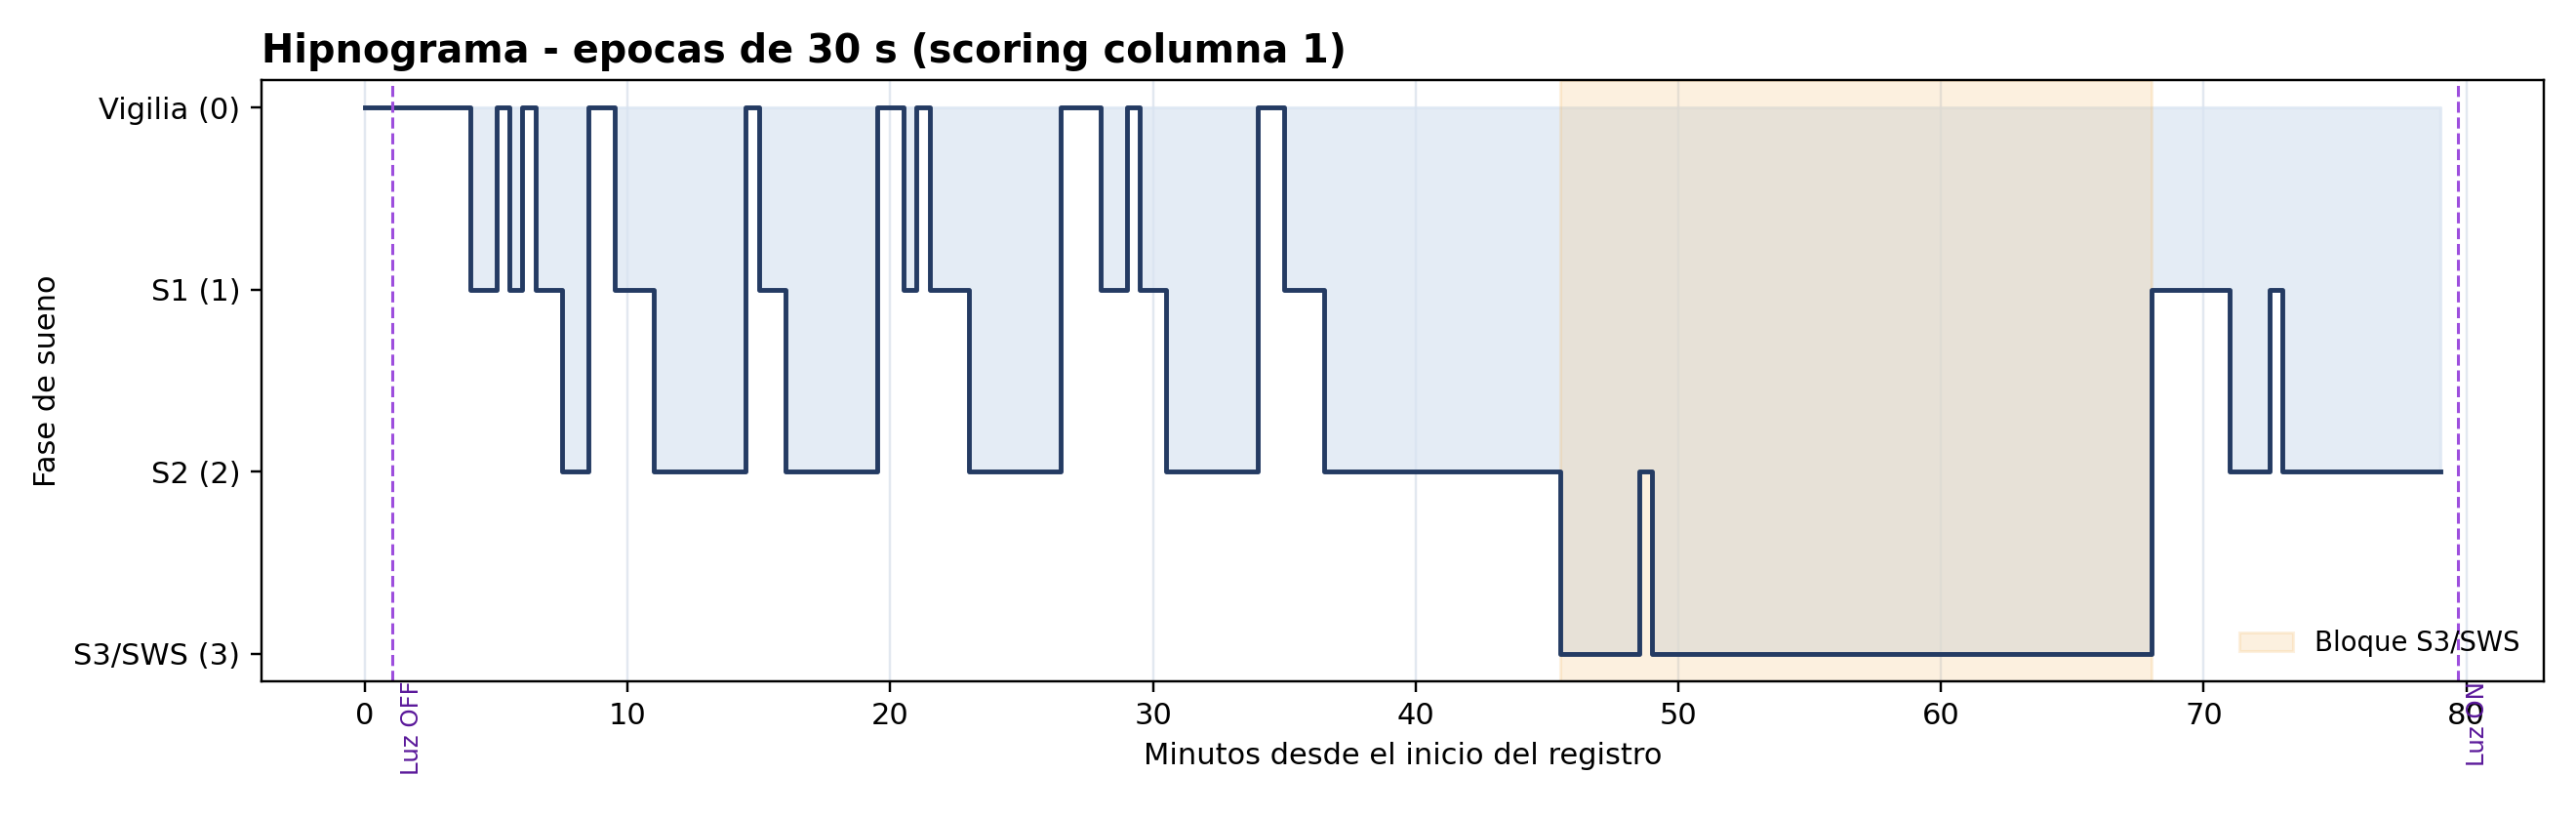
\includegraphics[width=\linewidth]{hipnograma_eeg.png}
\end{column}
\begin{column}{0.28\textwidth}
\begin{card}[bluecard]{\linewidth}
\textbf{Latencia de sueño}\par
4 min
\end{card}
\vspace{0.2cm}
\begin{card}[orangecard]{\linewidth}
\textbf{Latencia a S3}\par
45.5 min
\end{card}
\vspace{0.2cm}
\begin{card}[greencard]{\linewidth}
\textbf{Bloque SWS}\par
45.5-68 min
\end{card}
\vspace{0.2cm}
\begin{card}[whitecard]{\linewidth}
\textbf{REM}\par
No observado
\end{card}
\end{column}
\end{columns}
\source{Dataset BrainVision secundario; scoring en épocas de 30 s.}
\end{frame}

% 12
\begin{frame}{Tiempo por fase}{Predomina NREM, con casi 28\% del registro en S3/SWS.}
\begin{center}
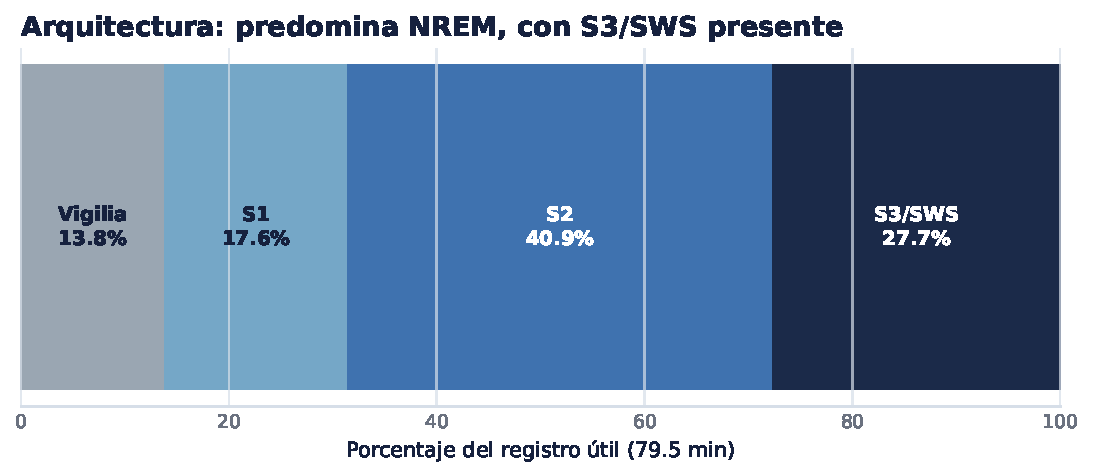
\includegraphics[height=0.42\textheight]{eeg_fases_distribucion.pdf}
\end{center}
\vspace{-0.05cm}
\small
\begin{columns}[T,totalwidth=\textwidth]
\begin{column}{0.24\textwidth}\begin{card}[whitecard]{\linewidth}\textbf{S2}\par 32.5 min\\40.9\%\end{card}\end{column}
\begin{column}{0.24\textwidth}\begin{card}[whitecard]{\linewidth}\textbf{S3/SWS}\par 22.0 min\\27.7\%\end{card}\end{column}
\begin{column}{0.24\textwidth}\begin{card}[whitecard]{\linewidth}\textbf{Sueño total}\par 68.5 min\end{card}\end{column}
\begin{column}{0.24\textwidth}\begin{card}[whitecard]{\linewidth}\textbf{Eficiencia}\par 86.2\%\end{card}\end{column}
\end{columns}
\source{Reporte EEG MNE v3 sobre dataset secundario.}
\end{frame}

% 13
\begin{frame}{Firma espectral: delta y sigma}{Los ritmos observados son compatibles con el marco de consolidación.}
\begin{columns}[T,totalwidth=\textwidth]
\begin{column}{0.49\textwidth}
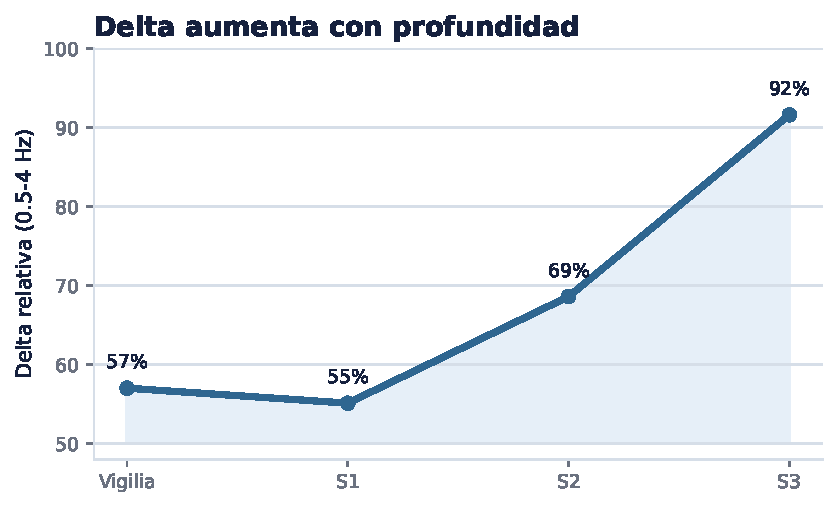
\includegraphics[width=\linewidth]{eeg_delta_relativa.pdf}
\end{column}
\begin{column}{0.49\textwidth}
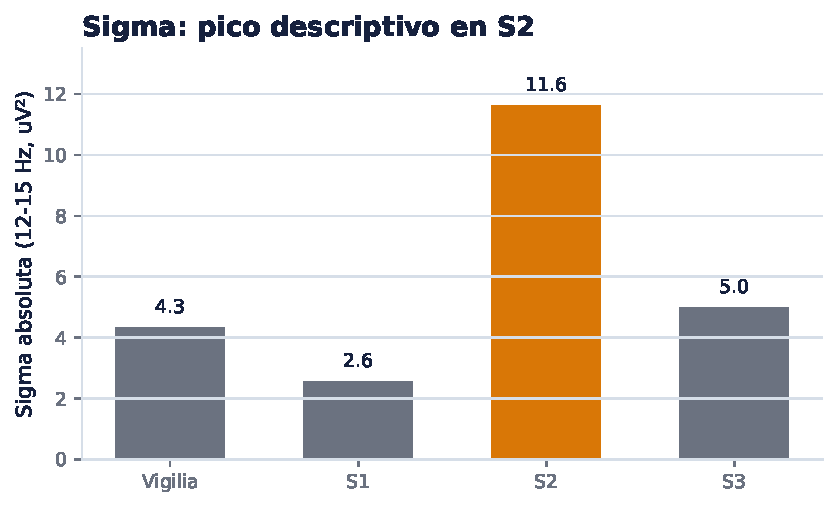
\includegraphics[width=\linewidth]{eeg_sigma_absoluta.pdf}
\end{column}
\end{columns}
\vspace{0.25cm}
\begin{card}[whitecard]{\textwidth}
Delta relativa aumenta hacia S3/SWS; sigma absoluta alcanza su pico en S2. Se reporta como potencia de banda, no como detección formal de husos.
\end{card}
\source{Welch sobre C3; bandas delta 0.5-4 Hz y sigma 12-15 Hz.}
\end{frame}

% 14
\begin{frame}{Qué podemos decir y qué no}{La honestidad metodológica sostiene la interpretación.}
\begin{columns}[T,totalwidth=\textwidth]
\begin{column}{0.48\textwidth}
\begin{card}[greencard]{\linewidth}
\textbf{Sí podemos decir}\par
\begin{itemize}
\item El EEG secundario muestra NREM con S3/SWS.
\item Hay potencia delta en S3 y sigma elevada en S2.
\item El patrón fisiológico es compatible con ritmos de consolidación.
\end{itemize}
\end{card}
\end{column}
\begin{column}{0.48\textwidth}
\begin{card}[orangecard]{\linewidth}
\textbf{No podemos decir}\par
\begin{itemize}
\item Que los husos de este EEG expliquen la memoria de esos sujetos.
\item Que haya prueba estadística o causal fuerte.
\item Que sigma sea huso confirmado sin detector formal.
\end{itemize}
\end{card}
\end{column}
\end{columns}
\vspace{0.5cm}
\claim{La relación memoria-EEG se presenta como integración teórica, no como correlación directa.}
\source{Restricción metodológica del práctico; guion de exposición; análisis propio.}
\end{frame}

% 15
\begin{frame}{Por qué el sujeto propio pudo no dormir}{Variables moduladoras plausibles, no causas confirmadas.}
\begin{columns}[T,totalwidth=\textwidth]
\begin{column}{0.62\textwidth}
\begin{columns}[T,totalwidth=\linewidth]
\begin{column}{0.48\linewidth}\begin{card}[bluecard]{\linewidth}\textbf{Proceso C / cronotipo}\par Siesta 16:00: posible contra-fase individual.\end{card}\end{column}
\begin{column}{0.48\linewidth}\begin{card}[orangecard]{\linewidth}\textbf{Cafeína}\par Antagoniza adenosina; podría elevar latencia.\end{card}\end{column}
\end{columns}
\vspace{0.25cm}
\begin{columns}[T,totalwidth=\linewidth]
\begin{column}{0.48\linewidth}\begin{card}[greencard]{\linewidth}\textbf{Estrés}\par Activación simpática/HPA dificulta conciliar.\end{card}\end{column}
\begin{column}{0.48\linewidth}\begin{card}[whitecard]{\linewidth}\textbf{Pantallas / luz}\par Puede retrasar fase circadiana.\end{card}\end{column}
\end{columns}
\vspace{0.25cm}
\begin{card}[whitecard]{\linewidth}\textbf{Ambiente y dispositivo}\par Dormir en laboratorio, con electrodos, puede aumentar incomodidad y vigilancia.\end{card}
\end{column}
\begin{column}{0.34\textwidth}
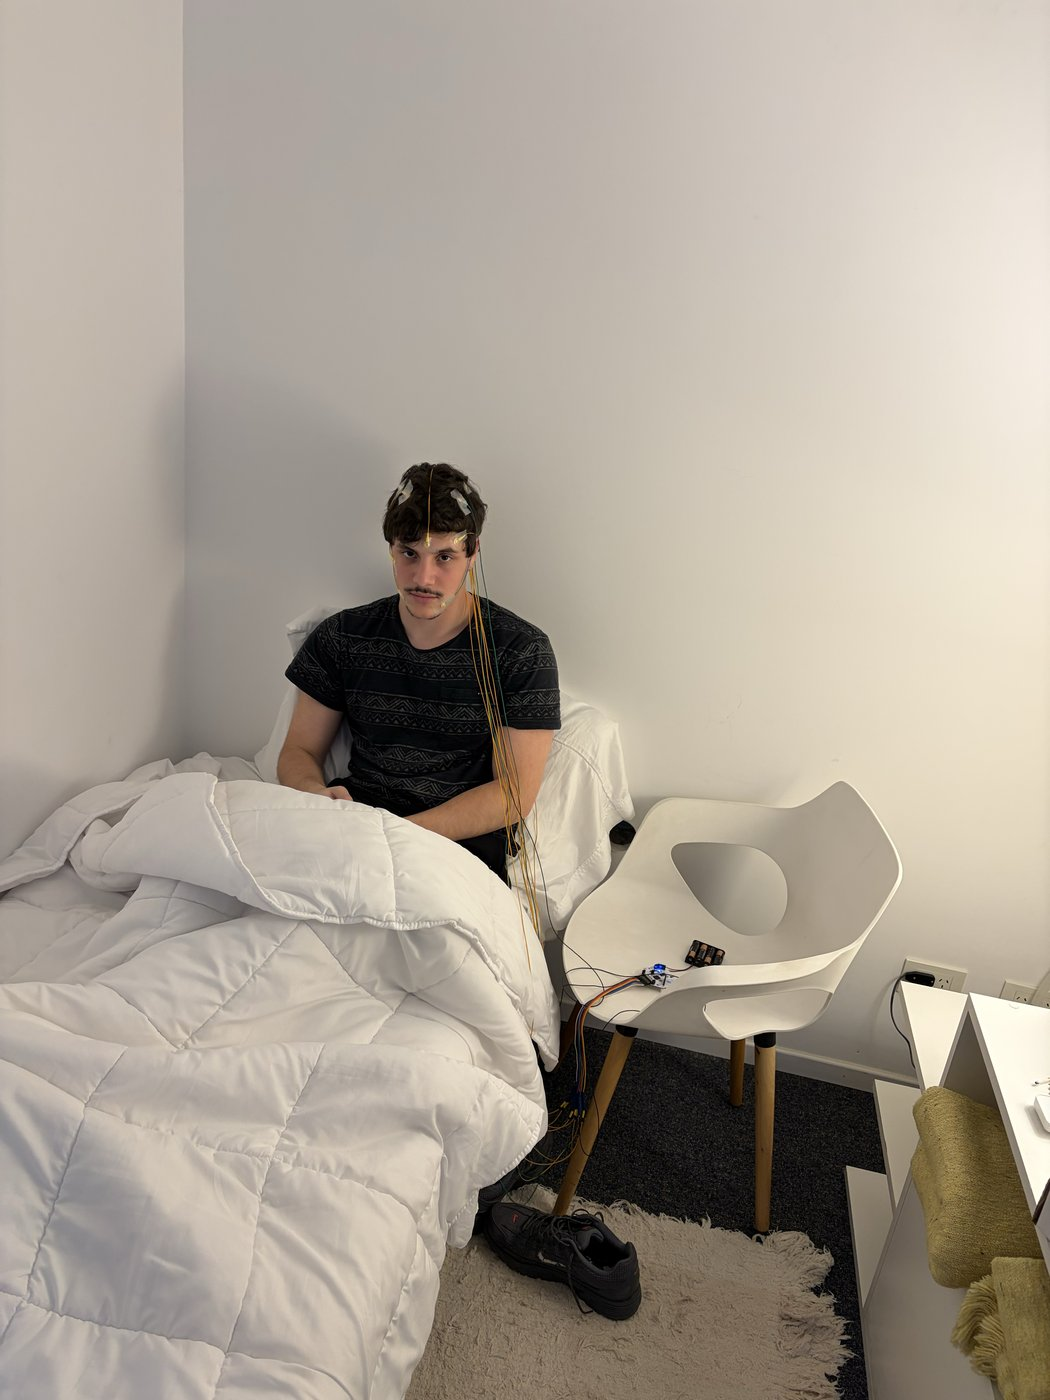
\includegraphics[height=0.62\textheight]{siesta_entorno.png}\par
\smallnote{Contexto de siesta experimental.}
\end{column}
\end{columns}
\source{Clases de ritmos circadianos, estrés, fármacos/cafeína e higiene del sueño.}
\end{frame}

% 16
\begin{frame}{Discusión integrada}{El trabajo encaja si se lee con límites claros.}
\begin{columns}[T,totalwidth=\textwidth]
\begin{column}{0.32\textwidth}\begin{card}[bluecard]{\linewidth}\textbf{Conducta}\par Mayor TS en sueño y mejora +2, pero con base inicial alta.\end{card}\end{column}
\begin{column}{0.32\textwidth}\begin{card}[orangecard]{\linewidth}\textbf{Fisiología}\par EEG secundario con S2 dominante, S3/SWS presente y sigma en S2.\end{card}\end{column}
\begin{column}{0.32\textwidth}\begin{card}[greencard]{\linewidth}\textbf{Teoría}\par Compatible con consolidación activa y homeostasis sináptica.\end{card}\end{column}
\end{columns}
\vspace{0.45cm}
\begin{card}[whitecard]{\textwidth}
\textbf{Limitaciones centrales:} condición sueño $n=1$; memoria y EEG de fuentes distintas; no hay S4 ni REM; sigma es proxy; no se infieren causas del no-sueño sin medición directa.
\end{card}
\source{Consigna oficial; clases teóricas; resultados conductuales y EEG.}
\end{frame}

% 17
\begin{frame}{Conclusión}{Respuesta directa a la pregunta inicial.}
\begin{center}
\begin{beamercolorbox}[wd=0.82\textwidth,sep=0.32cm,rounded=true]{darkcard}
{\LARGE \bfseries Compatible con la hipótesis; no demostración causal.}
\end{beamercolorbox}
\end{center}
\vspace{0.35cm}
\begin{columns}[T,totalwidth=\textwidth]
\begin{column}{0.48\textwidth}
\begin{card}[greencard]{\linewidth}
\textbf{Apoya descriptivamente}\par
Sujeto sueño: mayor desempeño final. EEG secundario: NREM con SWS y sigma en S2.
\end{card}
\end{column}
\begin{column}{0.48\textwidth}
\begin{card}[orangecard]{\linewidth}
\textbf{Qué falta para afirmar más}\par
Mismo sujeto con memoria + EEG, mayor $n$, control de moduladores y detector formal de husos.
\end{card}
\end{column}
\end{columns}
\vspace{0.35cm}
\centering\textbf{Cierre: apoyo descriptivo y parcial.}
\source{Síntesis del práctico y de las clases teóricas.}
\end{frame}

% 18
\begin{frame}{Apéndice técnico}{Datos para responder preguntas metodológicas.}
\begin{columns}[T,totalwidth=\textwidth]
\begin{column}{0.48\textwidth}
\begin{card}[whitecard]{\linewidth}
\textbf{EEG}\par
\begin{itemize}
\item BrainVision, 10 canales, 250 Hz.
\item C3 usado; C4 descartado.
\item Notch 50 Hz + pasa banda 0.3-35 Hz.
\item 159 épocas de 30 s sin solapamiento.
\end{itemize}
\end{card}
\end{column}
\begin{column}{0.48\textwidth}
\begin{card}[whitecard]{\linewidth}
\textbf{Bandas y fases}\par
\begin{itemize}
\item Delta 0.5-4; theta 4-8; alfa 8-12; sigma 12-15; beta 15-30 Hz.
\item Fases observadas: Vigilia, S1, S2, S3/SWS.
\item Sin S4 ni REM en el scoring usado.
\end{itemize}
\end{card}
\end{column}
\end{columns}
\vspace{0.35cm}
\begin{card}[bluecard]{\textwidth}
\textbf{Lenguaje recomendado:} ``compatible con'', ``apoyo descriptivo'', ``proxy de sigma''. Evitar: ``demostrado'', ``causal'', ``los husos explican el resultado''.
\end{card}
\source{Script de análisis EEG MNE v3; guion metodológico.}
\end{frame}

\end{document}
